% This document is distributed under the creative commons license:
% Attribution-ShareAlike 4.0 International (CC BY-SA 4.0)
% For the full license, see:
% http://creativecommons.org/licenses/by-sa/4.0/
\documentclass{beamer}

\usepackage{hyperref}
\usepackage{listings}
\usepackage{color}
\usepackage{minted}
\usepackage[normalem]{ulem}
\usepackage{beamerthemeOTS}

\title
{Design Patterns: an Introduction}

%\subtitle
%{Include Only If Paper Has a Subtitle}

\author[B. Bleuz\'e \and H. Schol] % (optional, use only with lots of authors)
{\textsc{Beno\^it Bleuz\'e} \and \textsc{Haiko Schol}}
% - Give the names in the same order as the appear in the paper.
% - Use the \inst{?} command only if the authors have different
%   affiliation.

\date[2014] % (optional, should be abbreviation of conference name)
{27/08/2014}

\subject{Design Patterns}

\definecolor{code_bg} {rgb}{0.95,0.95,0.95}

\begin{document}
\begin{frame}
  \titlepage
\end{frame}

\begin{frame}
\frametitle {Introduction}
  \textbf{Design Patterns}, what is all the fuss about?
\begin{itemize}
 \item Mantra uttered over and over by old bearded gurus
 \item Scary diagrams
 \item Abstract, mysterious names
 \item universal magical answer to the spaghetti code I end up having at the end of my project
\end{itemize}
\centering \only<2->{\alert {Let's demystify\dots}}
\end{frame}

\begin{frame}
  \frametitle{Outline}
  \tableofcontents
  % You might wish to add the option [pausesections]
\end{frame}

\section{Engineering techniques}
\begin{frame}
\frametitle {History}
\begin{itemize}
 \item \textbf{Design Patterns}: invented by \only<1>{software}\only <2->{\emph{\sout{software}}} Architect, \emph{Christopher Alexander}.\pause
 \item \pause \textbf{Design Patterns: Elements of Reusable Object-Oriented Software} 1994, \\
authored by the \textbf{Gang Of Four} (\emph{Erich Gamma, Richard Helm, Ralph Johnson and John Vlissides}) popularised the concept in Computer science.
 \item \pause Since then, countless books on how to apply many more patterns to many specific languages and problems.
\end{itemize}




\end{frame}
\begin{frame}
 \frametitle{Reusable techniques solving recurring problems}
They are \textbf{not}:
  \begin{itemize}
   \item tools (tools are editors or IDEs)
   \item ready made one size fits all solutions
  \end{itemize}
\end{frame}



\begin{frame}
\frametitle {Reusable techniques solving recurring problems}
A Pattern is only complete if it comes with:
\begin{itemize}
 \item a typical situation along with why it causes trouble
 \item a solution and the reason it is a good one.
 \item a context, when to apply it.
 \item limitations
\end{itemize}
\end{frame}

\section{Categories}

\begin{frame}
\frametitle {GoF Object Oriented Categories}
 In the book \textbf{Design Patterns}, the are the following categories:
\begin{description}
 \item [Creational] create resources instead of direct instantiation
 \item [Structural] organise the structure of the data: hierarchy, composition
 \item [Behavioral] drive the data flow, communication between objects
\end{description}
\end{frame}

\begin{frame}
\frametitle {GoF Creational Patterns}

\begin{description}
 \item [Abstract Factory] groups object factories that have a common theme.
 \item [Builder constructs] complex objects by separating construction and representation.
 \item [Factory Method] creates objects without specifying the exact class to create.
 \item [Prototype] creates objects by cloning an existing object.
 \item [Singleton] restricts object creation for a class to only one instance.
\end{description}
\end{frame}

\begin{frame}
\frametitle {GoF Structural Patterns}
\begin{small}
\begin{description}
 \item [Adapter] allows classes with incompatible interfaces to work together by wrapping its own interface around that of an already existing class.
 \item [Bridge] decouples an abstraction from its implementation so that the two can vary independently.
 \item [Composite] composes zero-or-more similar objects so that they can be manipulated as one object.
 \item [Decorator] dynamically adds/overrides behaviour in an existing method of an object.
 \item [Facade] provides a simplified interface to a large body of code.
 \item [Flyweight] reduces the cost of creating and manipulating a large number of similar objects.
 \item [Proxy] provides a placeholder for another object to control access, reduce cost, and reduce complexity.
\end{description}
\end{small}
\end{frame}

\begin{frame}
\frametitle {GoF Behavioral Patterns}

\begin{scriptsize}
\begin{description}
 \item [Chain of responsibility] delegates commands to a chain of processing objects.
 \item [Command] creates objects which encapsulate actions and parameters.
 \item [Interpreter] implements a specialized language.
 \item [Iterator] accesses the elements of an object sequentially without exposing its underlying representation.
 \item [Mediator] allows loose coupling between classes by being the only class that has detailed knowledge of their methods.
 \item [Memento] provides the ability to restore an object to its previous state (undo).
 \item [Observer] is a publish/subscribe pattern which allows a number of observer objects to see an event.
 \item [State] allows an object to alter its behavior when its internal state changes.
 \item [Strategy] allows one of a family of algorithms to be selected on-the-fly at runtime.
 \item [Template method] defines the skeleton of an algorithm as an abstract class, allowing its subclasses to provide concrete behavior.
 \item [Visitor] separates an algorithm from an object structure by moving the hierarchy of methods into one object.
\end{description}  
\end{scriptsize}
\end{frame}

\begin{frame}
\frametitle {Other known categories}

\begin{description}
 \item [Architectural] Large application scale patterns: core/plugin, data stores\dots
 \item [Concurrency] concurrent programming techniques, including locking mechanisms, thread pooling\dots
 \item [Testing] code testing patterns: mock objects, set-up/tear-down\dots
 \item [Domain specific] Some patterns are very much domain specific
\end{description}  
\end{frame}

\section{Concrete examples}

\subsection{MVC Pattern}
\begin{frame}
\frametitle{MVC: Principle}
\begin{center}
   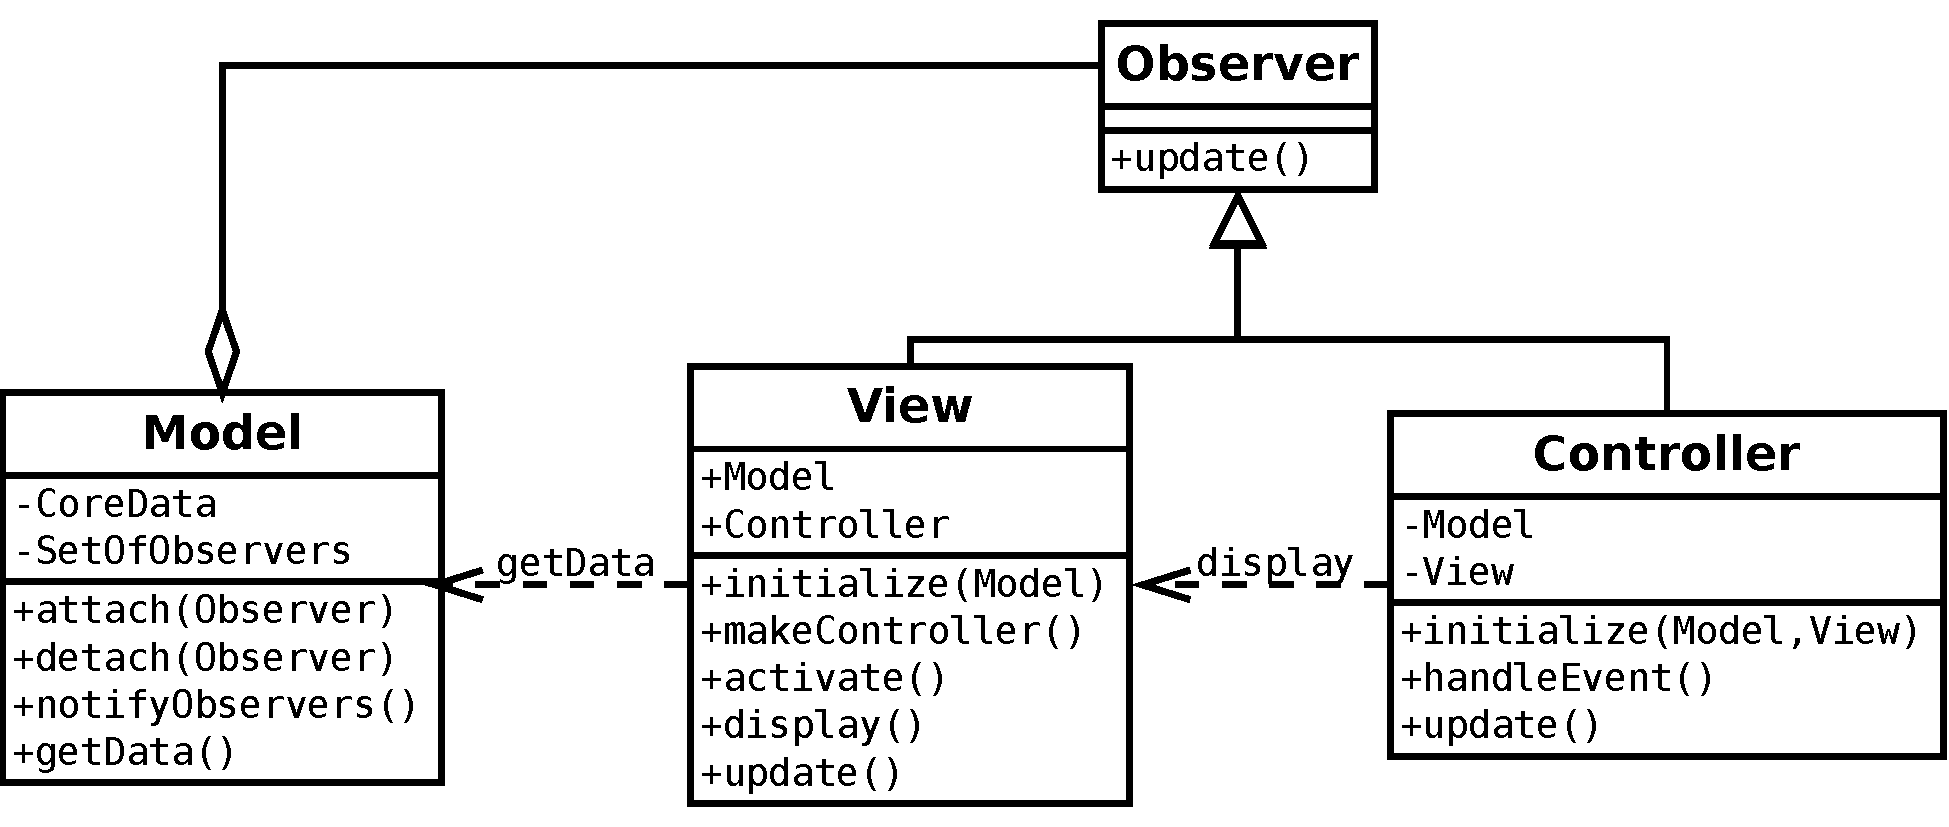
\includegraphics[width=\textwidth]{MVC.pdf}
\end{center}
\end{frame} 

\begin{frame}
\frametitle{MVC: Variations}
\begin{itemize}
 \item Qt uses \textbf{MV} pattern
 \item Django uses \textbf{MVT} pattern
 \item <only 2->Everybody's loose interpretation of "where do my controller stops and my view starts" 
\end{itemize}

\end{frame}

\subsection{Creational Patterns}
\begin{frame}
\frametitle{Factory Method Pattern: Principle}
\begin{center}
   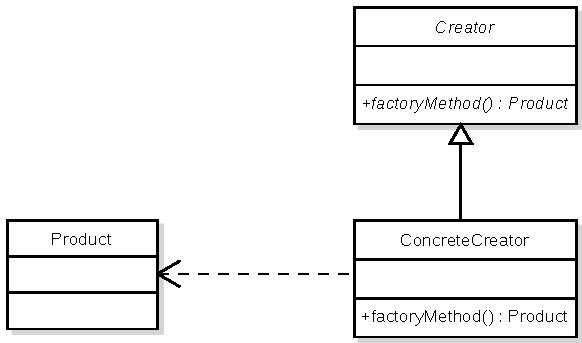
\includegraphics[width=\textwidth]{FactoryMethod.pdf}
\end{center}
\end{frame} 

\begin{frame}[fragile]
\frametitle{Factory Method Pattern: Code} 
\begin{minted} [fontsize=\footnotesize,bgcolor=code_bg] {python}
root = etree.Element('body')
h1 = etree.Element('h1')
h1.text = 'The Title'
root.append(h1)
p = etree.Element('p')
p.text = 'Always write Python'
root.append(p)

from lmxl.builder import E

doc = E('body',
        E('h1', 'The Title'),
        E('p', 'Always write Python'))
\end{minted}
\end{frame}

\subsection{Structural Patterns}

\begin{frame}
\frametitle{Adapter Pattern: Principle}
\begin{center}
   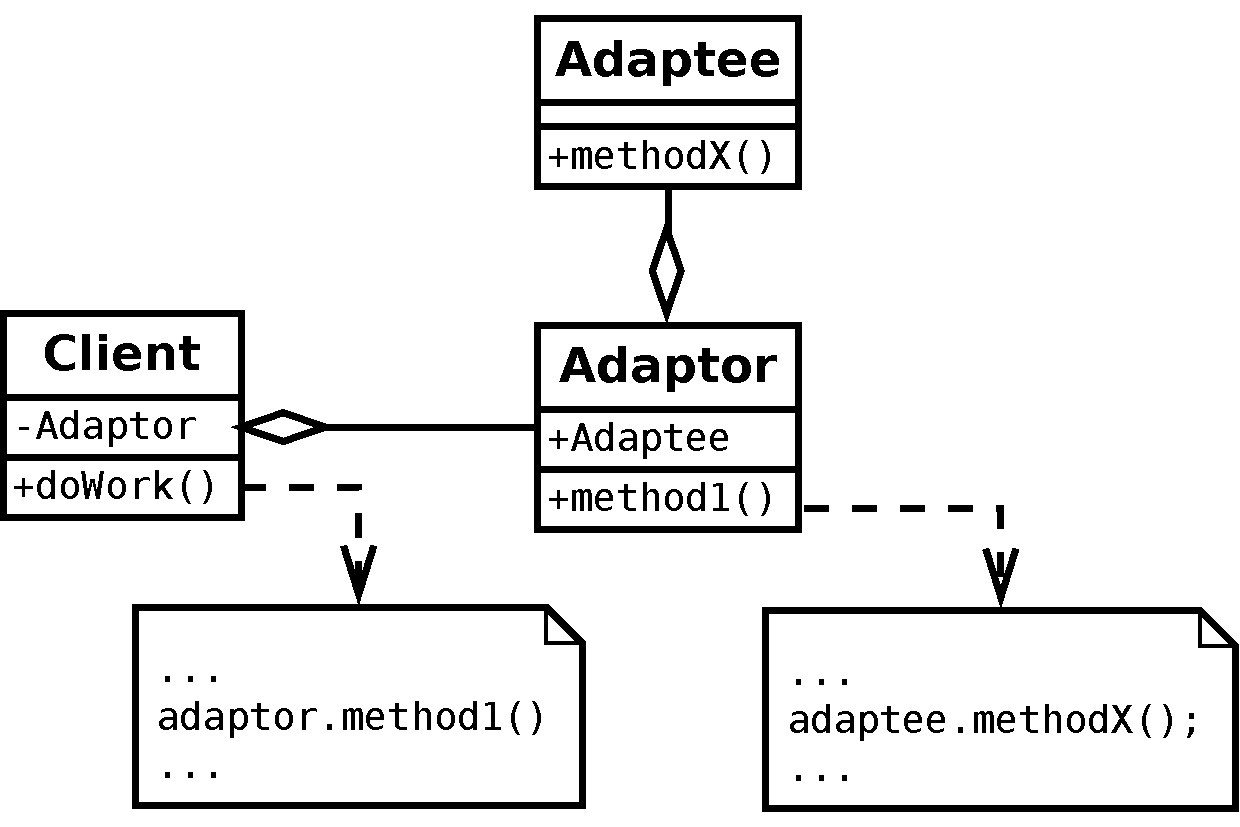
\includegraphics[width=.8\textwidth]{Adapter.pdf}
\end{center}
\end{frame} 

\begin{frame}[fragile]
\frametitle{Adapter Pattern: Code}
Python has the concept of a "file-like" object, which has read() and write(). Examples are \texttt{file} and \texttt{StringIO}, but \textbf{not} \texttt{socket} (it has \texttt{send()} and \texttt{recv()} instead). Luckily, we can get an Adapter from \texttt{socket} with \texttt{makefile()}:
\bigskip
\begin{minted} [fontsize=\footnotesize,bgcolor=code_bg] {python}
import socket

s = socket.socket(socket.AF_INET)
s.connect(...)
s.send('hello there')
file_like_socket = s.makefile()
file_like_socket.write('hi again')
\end{minted}
\end{frame}

\subsection{Behavioral Patterns}

\begin{frame}[fragile]
\frametitle{Command Pattern: Principle}
\begin{center}
   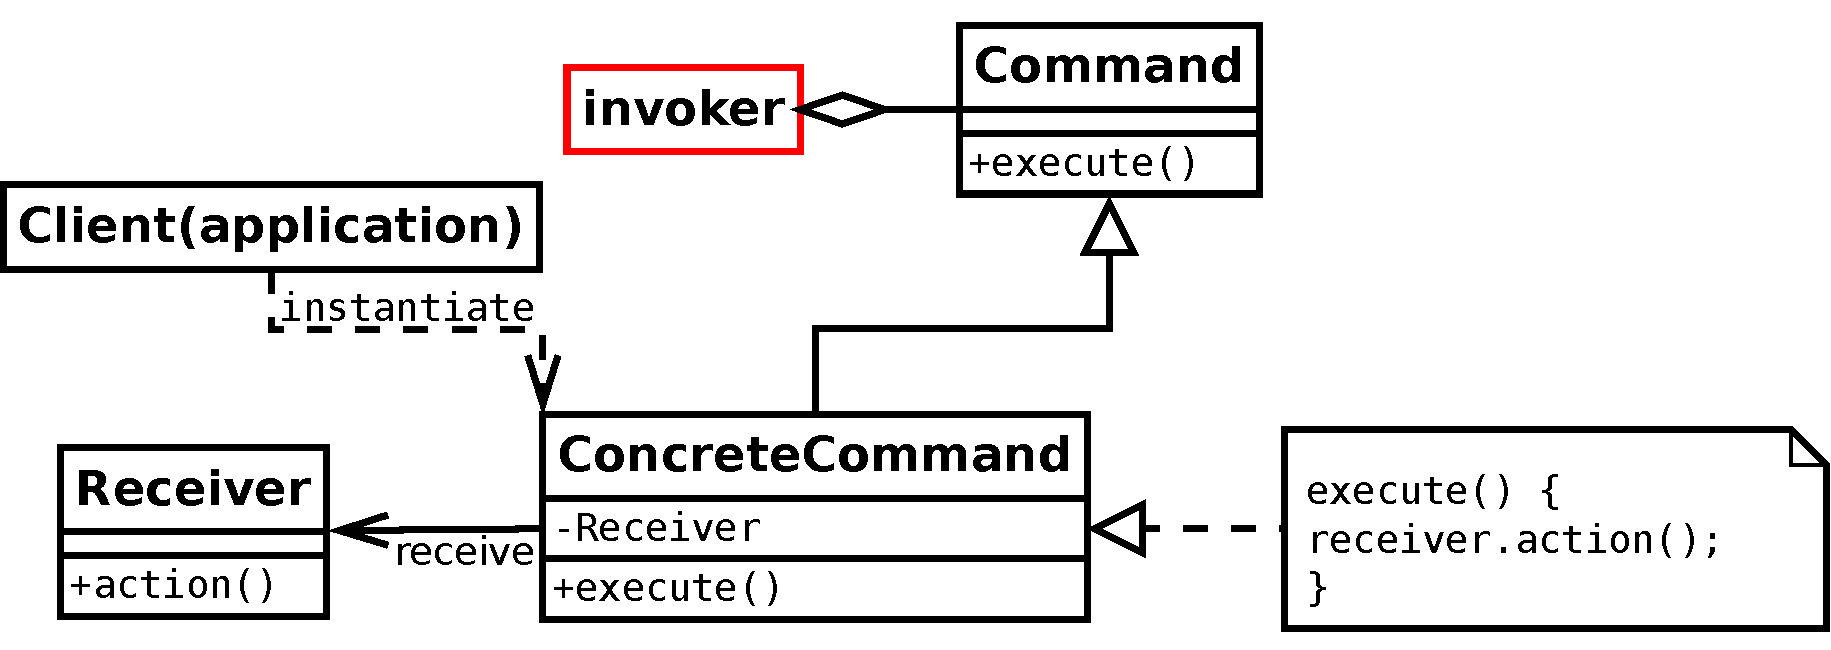
\includegraphics[width=\textwidth]{Command.pdf}
\end{center}
\end{frame}

\begin{frame}[fragile]
\frametitle{Command Pattern: Code} 
\begin{minted} [fontsize=\footnotesize,bgcolor=code_bg] {python}
def paint_line(x1, y1, x2, y2): pass

class PaintLineCommand(object):
  def __init__(self, x1, y1, x2, y2):
      self.x1, self.y1 = x1, y1
      self.x2, self.y2 = x2, y2

  def __call__(self):
      paint_line(self.x1, self.y1, self.x2, self.y2)

  def __str__(self):
      return 'paint_line from {}/{} to {}/{}'.format(
          self.x1, self.y1, self.x2, self.y2)

cmd = PaintLineCommand(5, 23, 42, 123)
cmd()
logging.debug(cmd)
\end{minted}
\end{frame}

\begin{frame}[fragile]
\frametitle{Command Pattern: Code} 
\begin{minted} [bgcolor=code_bg,fontsize=\footnotesize] {python}
class PaintLineCommand(object):
  # ...

  def undo(self):
      erase_line(self.x1, self.y1, self.x2, self.y2)


cmd = PaintLineCommand(5, 23, 42, 123)
cmd()
command_history.append(cmd)
command_history[-1].undo()
\end{minted}
\end{frame}

\begin{frame}[fragile]
\frametitle{Python Perspective}
Patterns don't have to be about object-oriented design. They can be something very simple.
\linebreak
\linebreak
\begin{minted}[fontsize=\footnotesize,bgcolor=code_bg]{python}
if 'page' in params:
    page = params['page']
else:
    page = 1
\end{minted}
\linebreak
Can be written as
\linebreak
\begin{minted}[fontsize=\footnotesize,bgcolor=code_bg]{python}
page = params.get('page', 1)
\end{minted}
\end{frame}

\section{WordS of Caution}
% language specific
% always evolving: trends and falls
\begin{frame}
 \frametitle{Limitations}
\begin{itemize}
 \item Language specific patterns
 \item Trends
 \item Technical advances, obsolescence
\end{itemize}
\end{frame}

\begin{frame}
\frametitle{Singleton Pattern: Principle}
\begin{itemize}
 \item One instance shared all over the code: "global object"
 \item Examples: config managers, Factories, Facade objects
\end{itemize}
\end{frame} 

\begin{frame}
\frametitle{Singleton Pattern: Python}
There are many ways to implement it in Python.
  \begin{itemize}
   \item a module instead of a class
   \item a class method instance() (does not enforce single instance)
   \item implement \_\_new\_\_()
   \item metaclass
   \item ...
   \item use the Monostate Pattern instead
  \end{itemize}
\end{frame}

\begin{frame}[fragile]
\frametitle{Singleton Pattern: IOLoop in Tornado}
\begin{footnotesize}
\begin{minted}[bgcolor=code_bg]{python}
@staticmethod
def instance():
    """Returns a global `IOLoop` instance.
       ...
    """
    if not hasattr(IOLoop, "_instance"):
        with IOLoop._instance_lock:
            if not hasattr(IOLoop, "_instance"):
                # New instance after double check
                IOLoop._instance = IOLoop()
    return IOLoop._instance
\end{minted}
\end{footnotesize}
\linebreak
Q: But is it thread-safe?
\end{frame}

\begin{frame}[fragile]
\frametitle{Singleton Pattern: Metaclass}
\begin{minted}[bgcolor=code_bg]{python}
class Singleton(type):
    def __init__(cls, name, bases, attrs):
        super(Singleton, cls).__init__(
            cls, bases, attrs)
        
        cls._instance = None

    def __call__(cls, *a, **k):
        if cls._instance is None:
            cls._instance = super(
                Singleton, cls).__call__(*a, **k)

        return cls._instance
\end{minted}
\end{frame}

\begin{frame}[fragile]
\frametitle{Singleton Pattern: Using the metaclass}
\begin{minted}[bgcolor=code_bg]{python}
class EventCounter(object):
    __metaclass__ = Singleton

    def __init__(self):
        self.count = 0

    def register_event(self):
        self.count += 1
\end{minted}

\begin{small}
\begin{verbatim}
>>> a, b = EventCounter(), EventCounter()
>>> b.count
0
>>> a.register_event()
>>> b.count
1
\end{verbatim}
\end{small}
\end{frame}

\begin{frame}[fragile]
\frametitle{Singleton Pattern: Alternative "Monostate"}
\begin{minted}[bgcolor=code_bg]{python}
class Borg(object):
    _shared_state = {}

    def __new__(cls, *a, **k):
        obj = super(Borg, cls).__new__(cls, *a, **k)
        obj.__dict__ = cls._shared_state
        return obj


class SevenOfNine(Borg): pass
\end{minted}
\end{frame}

\begin{frame}
\frametitle{Singleton Pattern: Controversies}
\begin{itemize}
 \item very much used, BUT
 \item introducing global state never encouraged
 \item tricky thread safety at initialisation (ultimately flawed in c++ due to uncertainty of dynamic loading order)
 \item overused: situations REALLY needing a singleton are rare
\end{itemize}
\end{frame} 

\section{Conclusions}
\begin{frame}
\frametitle{Conclusions}
Design patterns:
\begin{itemize}
  \item are recipes for solutions to common problems. 
  \item always come with descriptions of pb they solve, why they solve them, and the boundary conditions
  \item help engineers to speak and to code the same "language"
\end{itemize}

There is so much more we could have presented...
\end{frame}

\begin{frame}
\frametitle{Links}

  \begin{itemize}
   \item Many Python examples from here: https://www.youtube.com/watch?v=Er5K\_nR5lDQ
   \item Good talk by Alex Martelli at EuroPython: https://www.youtube.com/watch?v=bPJKYrZjq10
   \item \textbf{Design Patterns: Elements of Reusable Object-Oriented Software} 1994, \\
authored by \emph{Erich Gamma, Richard Helm, Ralph Johnson and John Vlissides}
  \end{itemize}

\end{frame}

 \begin{frame}
 \frametitle{Questions?}
 \begin{center}
 %   \includegraphics[height=.5\textheight]{Code-Refactoring-Cat-in-Bathtub.gif}
 % look at animate.
 \end{center}
 \end{frame}

\end{document}
